\section{Mission B}
	\subsection{Sous-mission B1}

	\begin{vwcol}[widths={0.8,0.2}, rule=0pt]
	\begin{minipage}{0.7\textwidth}
	\paragraph{Objectifs de la mission}

	L'objectif de cette mission était de travailler l'image de Gliese 667Cc afin de faire apparaître son atmosphère sur les images prises par une sonde, cette image étant de mauvaise qualité. 
	\end{minipage}
	\begin{minipage}{0.2\textwidth}
		\begin{flushright}
			\paragraph{Filtre utilisé}
		Egalisation
		\end{flushright}
	\end{minipage}
	\end{vwcol} 

	\begin{figure}[h]
	\centering
		\begin{multicols}{2}
		
\includegraphics[scale=0.525]{images/Gliese667Cc.png}
		Avant
		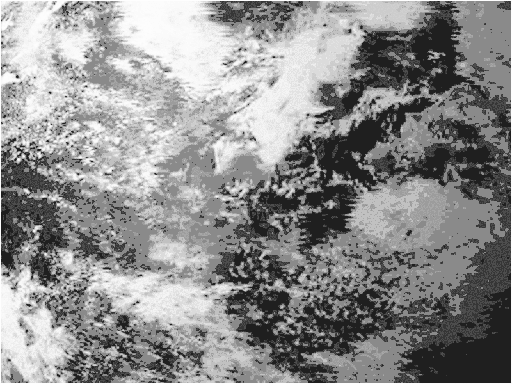
\includegraphics[scale=0.525]{images/Gliese667CcAFTER.png}
		Après
		\end{multicols}
	\end{figure}
	\vspace{-0.9cm}

		\paragraph{Procédé}	
			Pour cette mission une \emph{égalisation} a été réalisée sur cette image. Cette méthode fait nettement apparaître l'atmosphère de la planète. Une \emph{normalisation} avait été réalisée en premier lieu, qui faisait aussi apparaître cette atmosphère mais moins nettement.